\documentclass[10pt,aspectratio=169]{beamer}
\usepackage{tikz}
\usepackage[utf8]{inputenc}
%\usepackage[T1]{fontenc}
\usepackage[english]{babel}
%\usepackage[latin1]{inputenc}
%\usepackage[T1]{fontenc}
\usepackage{verbatim}
\usepackage{listings}

\lstset{
  language=C++,                 % the language of the code
  backgroundcolor=\color{white},   % choose the background color; you must add \usepackage{color} or \usepackage{xcolor}
  basicstyle=\footnotesize,        % the size of the fonts that are used for the code
  breakatwhitespace=false,         % sets if automatic breaks should only happen at whitespace
  breaklines=true,                 % sets automatic line breaking
  keywordstyle=\color{blue},       % keyword style
  captionpos=b,                    % sets the caption-position to bottom
  commentstyle=\color{blue},       % comment style
  deletekeywords={},            % if you want to delete keywords from the given language
  escapeinside={\%*}{*)},          % if you want to add LaTeX within your code
  extendedchars=true,              % lets you use non-ASCII characters; for 8-bits encodings only, does not work with UTF-8
  frame=single,                    % adds a frame around the code
  keepspaces=true,                 % keeps spaces in text, useful for keeping indentation of code (possibly needs columns=flexible)
  morekeywords={using, static_assert},            % if you want to add more keywords to the set
  numbers=left,                    % where to put the line-numbers; possible values are (none, left, right)
  numbersep=10pt,                   % how far the line-numbers are from the code
  numberstyle=\tiny\color{black}, % the style that is used for the line-numbers
  rulecolor=\color{black},         % if not set, the frame-color may be changed on line-breaks within not-black text (e.g. comments (green here))
  showspaces=false,                % show spaces everywhere adding particular underscores; it overrides 'showstringspaces'
  showstringspaces=false,          % underline spaces within strings only
  showtabs=false,                  % show tabs within strings adding particular underscores
  stepnumber=1,                    % the step between two line-numbers. If it's 1, each line will be numbered
  stringstyle=\color{red},     % string literal style
  tabsize=2,                       % sets default tabsize to 2 spaces
  title=\lstname                   % show the filename of files included with \lstinputlisting; also try caption instead of title
}

%\makeatletter
%\define@key{beamerframe}{t}[true]{% top
%\beamer@frametopskip=.2cm plus .5\paperheight\relax%
%\beamer@framebottomskip=0pt plus 1fill\relax%
%\beamer@frametopskipautobreak=\beamer@frametopskip\relax%
%\beamer@framebottomskipautobreak=\beamer@framebottomskip\relax%
%\def\beamer@initfirstlineunskip{}%
%}
%\makeatother   

%__________________________________________________________

% Possible themes

%\usetheme{AnnArbor}       % Bad color
%\usetheme{Antibes}       % Not good
%\usetheme{Bergen}        % Wastes space
%\usetheme{Berkeley}      % Very good
%\usetheme{Berlin}        % Very good
%\usetheme{Boadilla}      % Good
%\usetheme{CambridgeUS}   % Very good but no section list
%\usetheme{Copenhagen}    %  Limpo
%\usetheme{Dresden}       %  Vale a pena tambem
%\usetheme{Frankfurt}     % limpo, com lista mas sem pagina
%\usetheme{Goettingen}    % Lista de secoes na lateral esquerda
%\usetheme{Hannover}      %  Lista de secoes na lateral direita sem pagina
%\usetheme{Ilmenau}       % Com secao e sub
%\usetheme{JuanLesPins}   % Mais ou menos
%\usetheme{Luebeck}       % Limpo e bem organizado
\usetheme{Madrid}        % So titulo e com pagina
%\usetheme{Malmoe}        % Nao tem caixa para o titulo
%\usetheme{Marburg}       % Bem organizado, sem caixa pra titulo e com lista na direita
%\usetheme{Montpellier}   % Nao gosto do design
%\usetheme{PaloAlto}      % Boa escolha
%\usetheme{Pittsburgh}    % Fraco
%\usetheme{Rochester}     % So caixa pro titulo
%\usetheme{Singapore}     % Fraco
%\usetheme{Szeged}        % Legal
%\usetheme{Warsaw}        % Bom
%\usetheme{boxes}         % Fraco
%\usetheme{default}       % Fraco
%__________________________________________________________

% Possible color themes

%\usecolortheme{albatross}
\usecolortheme{beaver}         % Acho que é esse.
%\usecolortheme{beetle}        % Bom mas escuro
%\usecolortheme{crane}         % muito boa    
%\usecolortheme{default}        
%\usecolortheme{dolphin}      
%\usecolortheme{dove}          % legal
%\usecolortheme{fly}    
%\usecolortheme{lily}       
%\usecolortheme{orchid}       
%\usecolortheme{seagull}       % excelente mas cinza
%\usecolortheme{seahorse}     
%\usecolortheme{sidebartab}    
%\usecolortheme{whale}       
%\usecolortheme{wolverine}       

\colorlet{nodeU}{red!80!black}
\colorlet{nodeD}{red!80!black}
\colorlet{nodeO}{red!80!black}
\colorlet{value}{yellow!50!black}
\colorlet{dgfile}{red!80!black}

\tikzstyle{dgfile}=[draw,fill=dgfile,shape=rectangle,minimum width=2cm,inner sep=1ex]
\tikzstyle{nodeU}=[draw,fill=nodeU,shape=rectangle,minimum width=0.5cm  ,inner sep=1ex]
\tikzstyle{nodeD}=[draw,fill=nodeD,shape=rectangle,minimum width=1cm  ,inner sep=1ex]
\tikzstyle{nodeQ}=[draw,fill=nodeD,shape=rectangle,minimum width=2cm  ,inner sep=1ex]
\tikzstyle{nodeO}=[draw,fill=nodeO,shape=rectangle,minimum width=4cm  ,inner sep=1ex]
\tikzstyle{valueU}=[draw,fill=value,shape=rectangle,minimum width=0.5cm,inner sep=1ex]
\tikzstyle{valueD}=[draw,fill=value,shape=rectangle,minimum width=1cm,inner sep=1ex]
\tikzstyle{valueQ}=[draw,fill=value,shape=rectangle,minimum width=2cm,inner sep=1ex]
\tikzstyle{valueO}=[draw,fill=value,shape=rectangle,minimum width=4cm,inner sep=1ex]

\def\dgfile{\node[style=dgfile]}
\def\nodeU{\node[style=nodeU]}
\def\nodeD{\node[style=nodeD]}
\def\nodeQ{\node[style=nodeQ]}
\def\nodeO{\node[style=nodeO]}
\def\valueU{\node[style=valueU]}
\def\valueD{\node[style=valueD]}
\def\valueQ{\node[style=valueQ]}
\def\valueO{\node[style=valueO]}

%__________________________________________________________
% Apenas para o tema madrid

\defbeamertemplate*{footline}{my infolines theme}
{
  \leavevmode%
    \hbox{%
      \begin{beamercolorbox}[wd=.333333\paperwidth,ht=2.25ex,dp=1ex,center]{author in head/foot}%
        \usebeamerfont{author in head/foot}\insertshortauthor~~\insertshortinstitute
        \end{beamercolorbox}%
        \begin{beamercolorbox}[wd=.333333\paperwidth,ht=2.25ex,dp=1ex,center]{title in head/foot}%
        \usebeamerfont{title in head/foot}\insertshorttitle
        \end{beamercolorbox}%
        \begin{beamercolorbox}[wd=.333333\paperwidth,ht=2.25ex,dp=1ex,right]{date in head/foot}%
        \usebeamerfont{date in head/foot}\insertshortdate{}\hspace*{2em}
      \insertframenumber{} / \inserttotalframenumber\hspace*{2ex}
      \end{beamercolorbox}}%
        \vskip0pt%
}
%__________________________________________________________

\mode<presentation>
{
  %\setbeamercovered{transparent}
   %\setbeamertemplate{footline}[frame number]
  % or whatever (possibly just delete it)
}

\title[] {Node allocation}

\subtitle[] {How can we improve \texttt{C++} memory menagement}

\author[] {Marcelo Zimbres}

\institute[Marcelo Zimbres - Software Developer - Physicist]
{
  Presentation to WG21-SG14
}

\date[15 October 2016 - Magstadt - Germany] {14 October 2016 - Magstadt}

\subject{Node allocation 3}

% If you have a file called "university-logo-filename.xxx", where xxx
% is a graphic format that can be processed by latex or pdflatex,
% resp., then you can add a logo as follows:

%\pgfdeclareimage[height=1.2cm]{Wavelet}{fig/skymapJ8j2N127.pdf}
%\logo{\pgfuseimage{Wavelet}}

% Delete this, if you do not want the table of contents to pop up at
% the beginning of each subsection:
\AtBeginSubsection[]
{
  \begin{frame}<beamer>{Outline}
    \tableofcontents[currentsection,currentsubsection]
  \end{frame}
}

% If you wish to uncover everything in a step-wise fashion, uncomment
% the following command: 

%\beamerdefaultoverlayspecification{<+->}

\begin{document}

\begin{frame}
  \titlepage
\end{frame}

\begin{frame}{Outline}
  \tableofcontents[pausesections]
  % You might wish to add the option [pausesections]
\end{frame}

% Since this a solution template for a generic talk, very little can
% be said about how it should be structured. However, the talk length
% of between 15min and 45min and the theme suggest that you stick to
% the following rules:  

% - Exactly two or three sections (other than the summary).
% - At *most* three subsections per section.
% - Talk about 30s to 2min per frame. So there should be between about
%   15 and 30 frames, all told.

\begin{frame}[t]{Target audience - Goals}{}
\begin{columns}
\begin{column}{0.5\textwidth}
Goals.
\begin{itemize}
    \item Provide building blocks to memory allocation
    \item Use static type information to improve memory management
    \item Reduce memory footprint of linked data structures
    \item Reduce dependency on global state and on undefined behaviour
    \item Allow fine tunning
    \item Reduce complexity
\end{itemize}
\end{column}

\begin{column}{0.5\textwidth}
Target audience
\begin{itemize}
    \item Realtime/embedded programming.
    \item Games, high performace, 24/7 availability.
    \item Should be usefull for c++ programmers in general.
    \item Implementation available on github.
\end{itemize}
\end{column}
\end{columns}
\end{frame}

\part{Node allocation}

\section{Review of memory allocations \texttt{C++} containers}

\begin{frame}[fragile]{\texttt{C++} Allocators}
\begin{columns}
\begin{column}{0.5\textwidth}
\begin{itemize}
\item Abstraction to memory allocation inside containers.
\item All containers with dynamic size request memory from
their allocator internally.
\item The allocator is part of the container type.
\item Containers do not interact directly with the allocator but with
\texttt{std::allocator\_traits}.
\end{itemize}
\end{column}

\begin{column}{0.5\textwidth}
Part of the type.
\begin{lstlisting}
template<class T, class Allocator>
class list;
\end{lstlisting}

Basic usage
\begin{lstlisting}
std::allocator<int> alloc;
auto* p = alloc.allocate(n);
alloc.deallocate(p, n);
\end{lstlisting}
\end{column}
\end{columns}
\end{frame}

\section{Allocation patterns}

\begin{frame}{Containers and their allocation patterns}
\begin{columns}
\begin{column}{0.5\textwidth}
Array allocation only (i.e. runtime n)
\begin{itemize}
\item \texttt{std::vector}
\end{itemize}

Node allocation only (i.e. compile time n)
\begin{itemize}
\item \texttt{std::list}
\item \texttt{std::forward\_list}
\item \texttt{std::set}
\item \texttt{std::multiset}
\item \texttt{std::map}
\item \texttt{std::multimap}
\end{itemize}
\end{column}

\begin{column}{0.5\textwidth}
Both node and array allocation.
\begin{itemize}
\item \texttt{std::deque}
\item \texttt{std::unordered\_set}
\item \texttt{std::unordered\_multiset}
\item \texttt{std::unordered\_map}
\item \texttt{std::unordered\_multimap}
\end{itemize}
Summary
\begin{itemize}
\item 11 perform node allocation.
\item 6 perform exclusively node-allocation.
\item 5 perform both node and array allocation.
\item Node allocation is pretty common.
\end{itemize}

\end{column}
\end{columns}
\end{frame}

\begin{frame}[]{Allocation strategies}
{\texttt{malloc}, \texttt{jemalloc}, \texttt{tcmalloc},
\texttt{nedmalloc}, \texttt{hoard}, etc}
\begin{columns}
\begin{column}{0.5\textwidth}
Typical goals
\begin{itemize}
\item<alert@1> Avoid fragmentation. Improve locality.
\item<alert@2> Small sizes: Up $170$ pre-allocated lists.
\item<alert@3> Large sizes: Best fit, rounding on memory pages.
\item<alert@4> Avoid serialization on cuncurrent calls.
\item<alert@5> Bookkeeping information on blocks.
\item<alert@2> Rounding allocation sizes to fit pre-allocated buffers.
\end{itemize}

\end{column}

\begin{column}{0.5\textwidth}
Thoughts
\begin{itemize}
\item<alert@1> Hang same-size allocations on different pre-linked buffers.
\item<alert@2> Sizes are known at compile time. We can avoid this.
\item<alert@3> Do not use a global allocator.
\item<alert@4> Not needed if blocks have alway the same size.
\end{itemize}

\end{column}
\end{columns}
\end{frame}

\begin{frame}{Should node allocation be standardized}{Proposal to the ISO \texttt{C++} Standards Committee}
\vspace{-3cm}
    \begin{center}
        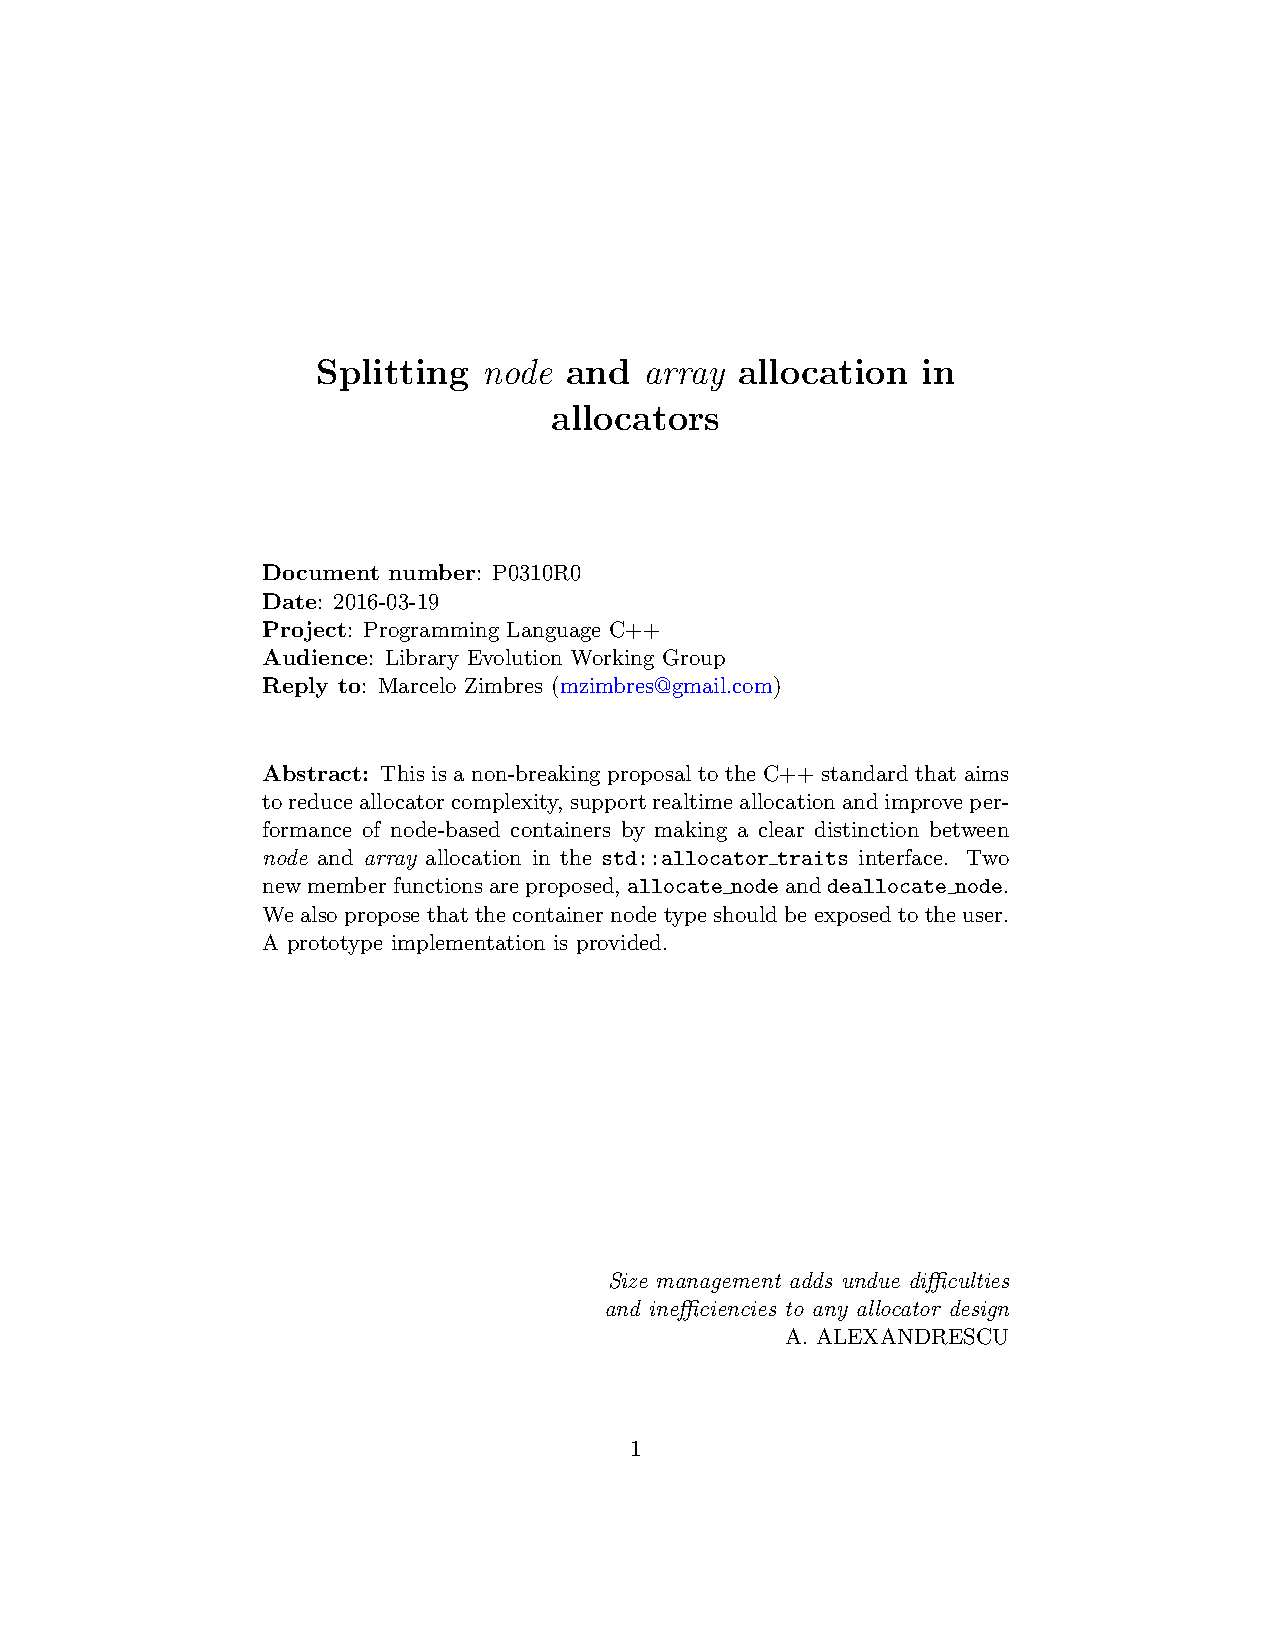
\includegraphics[scale=0.6]{fig/prop1.pdf} \\
    \end{center}
\end{frame}

\section{Node allocation}

\begin{frame}[t]{Containers and their allocation patterns}
\begin{columns}
\begin{column}{0.5\textwidth}

Node Allocation

\begin{itemize}
\item Simple and straighforward implementation.
\item Suitable for realtime/embedded.
\item Reduces memory fragmentation.
\item Basic building block used in array allocations as well.
\end{itemize}

\end{column}

\begin{column}{0.5\textwidth}
\begin{enumerate}
\item<alert@2> Get $N$ nodes at once.
\item<alert@3> Link them as a stack.
\item<alert@4> Repeat if more nodes are inserted.
\end{enumerate}

\end{column}
\end{columns}

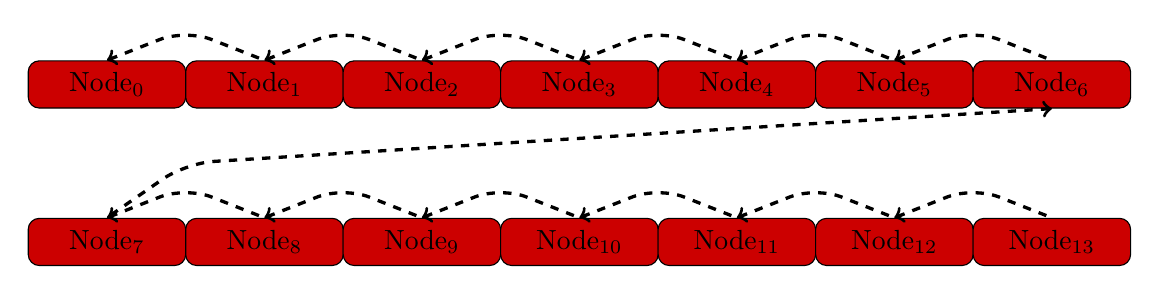
\begin{tikzpicture}[scale=1.0, rounded corners]

   \uncover<2-> {
      \dgfile (node0) at (-5.0,4) {Node$_0$};
      \dgfile (node1) at (-3.0,4) {Node$_1$};
      \dgfile (node2) at (-1.0,4) {Node$_2$};
      \dgfile (node3) at (1.0,4) {Node$_3$};
      \dgfile (node4) at (3.0,4) {Node$_4$};
      \dgfile (node5) at (5.0,4) {Node$_5$};
      \dgfile (node6) at (7.0,4) {Node$_6$};
   }

   \uncover<3-> {
      \draw[very thick,<-,dashed, rounded corners=10pt,color=black] (node0.north) -- (-4,4.7) -- (node1.north);
      \draw[very thick,<-,dashed, rounded corners=10pt,color=black] (node1.north) -- (-2,4.7) -- (node2.north);
      \draw[very thick,<-,dashed, rounded corners=10pt,color=black] (node2.north) -- ( 0,4.7) -- (node3.north);
      \draw[very thick,<-,dashed, rounded corners=10pt,color=black] (node3.north) -- ( 2,4.7) -- (node4.north);
      \draw[very thick,<-,dashed, rounded corners=10pt,color=black] (node4.north) -- ( 4,4.7) -- (node5.north);
      \draw[very thick,<-,dashed, rounded corners=10pt,color=black] (node5.north) -- ( 6,4.7) -- (node6.north);
   }

   \uncover<4-> {

      \dgfile (node7) at (-5.0,2) {Node$_{7}$};
      \dgfile (node8) at (-3.0,2) {Node$_{8}$};
      \dgfile (node9) at (-1.0,2) {Node$_{9}$};
      \dgfile (node10) at ( 1.0,2) {Node$_{10}$};
      \dgfile (node11) at ( 3.0,2) {Node$_{11}$};
      \dgfile (node12) at ( 5.0,2) {Node$_{12}$};
      \dgfile (node13) at ( 7.0,2) {Node$_{13}$};
   }

   \uncover<5-> {

      \draw[very thick,<-, dashed, rounded corners=10pt,color=black] (node6.south) --  (-4,3) --  (node7.north);
      \draw[very thick,<-, dashed, rounded corners=10pt,color=black] (node7.north) --  (-4,2.7) -- (node8.north);
      \draw[very thick,<-, dashed, rounded corners=10pt,color=black] (node8.north) --  (-2,2.7) -- (node9.north);
      \draw[very thick,<-, dashed, rounded corners=10pt,color=black] (node9.north) --  ( 0,2.7) -- (node10.north);
      \draw[very thick,<-, dashed, rounded corners=10pt,color=black] (node10.north) -- ( 2,2.7) -- (node11.north);
      \draw[very thick,<-, dashed, rounded corners=10pt,color=black] (node11.north) -- ( 4,2.7) -- (node12.north);
      \draw[very thick,<-, dashed, rounded corners=10pt,color=black] (node12.north) -- ( 6,2.7) -- (node13.north);
   }
\end{tikzpicture}


\end{frame}

\begin{frame}[fragile]{Array Allocation}
Array allcation
\begin{itemize}
\item Many possible strategies. Which one should I use?
\item Has to handle different sizes.
\item No silver bullet. Every problem requires a different approach.
\item Users do not want to care about this unless there is need.
\item malloc: suitable for large memory blocks, overused, hundreds of
\item LOC, system calls, etc.
\item May use node allocation as a building block.
\end{itemize}

\end{frame}

\begin{frame}[transparent]{Node sizes according to the number of elements needed}
\begin{columns}
\begin{column}{0.5\textwidth}
\begin{enumerate}
\item<alert@1> $N \le 256$ with $T \in [0, 256]$
\item<alert@2> $N \le 2^{16}$ with $T \in [0, 2^{16}]$
\item<alert@3> $N \le 2^{32}$ with $T \in [0, 2^{32}]$
\item<alert@4> $N \le 2^{64}$ with $T \in [0, 2^{64}]$
\end{enumerate}

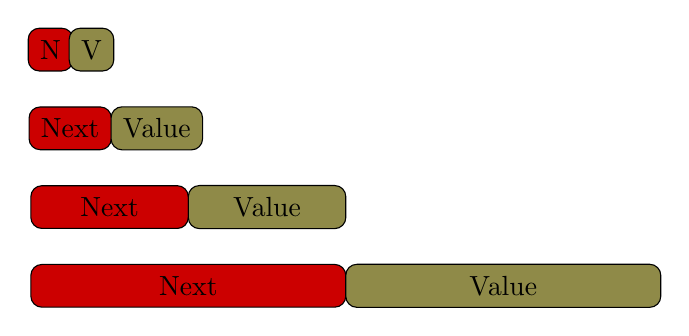
\begin{tikzpicture}[scale=1.0, rounded corners]

   \uncover<1-> {
      \nodeU (next) at (0.25,5) {N};
      \valueU (value) at (0.77,5) {V};
   }

   \uncover<2-> {
      \nodeD (next) at (0.5,4) {Next};
      \valueD (value) at (1.6,4) {Value};
   }

   \uncover<3-> {
      \nodeQ (next) at (1,3) {Next};
      \valueQ (value) at (3,3) {Value};
   }
   \uncover<4-> {
      \nodeO (next) at (2,2) {Next};
      \valueO (value) at (6,2) {Value};
   }
\end{tikzpicture}

\end{column}
\begin{column}{0.5\textwidth}

\begin{itemize}
\item The underlying data structure is a deque.
\item We do not have to address nodes with pointers.
\item For less than $256$ elements a \texttt{char} has enough bits.
\end{itemize}

\end{column}
\end{columns}

\end{frame}

%\begin{frame}{Cache Hierarchy - Latency}{Why it is important to reduce memory usage}
%    \begin{columns}
%        \begin{column}{0.4\textwidth}
%            Intel Haswell Mobile 
%            \begin{itemize}
%                \item Register: Fastest
%                \item L0: 6 KiB
%                \item L1: 128 KiB - 700 GiB/s
%                \item L2: 1 MiB - 200 GiB/s
%                \item L3: 6 MiB - 100 GB/s
%                \item L4: 128 MiB - 40 GB/s
%                \item Main memory – GiB - 10 GB/s
%            \end{itemize}
%        \end{column}
%
%        %\begin{column}{0.6\textwidth}
%        %    \begin{center}
%        %        \includegraphics[scale=0.7]{fig/cache.jpg} \\
%        %    \end{center}
%        %\end{column}
%    \end{columns}
%\end{frame}

\begin{frame}[fragile]{Linked list travesal illustration}
\begin{columns}
\begin{column}{0.6\textwidth}
Can we avoid pointers chasing?
\begin{enumerate}
\item<alert@1> Initial memory state. Available memory.
\item<alert@2> After insertion and removal we have chaos.
\item<alert@3> Traversal chasing pointers jumps to slow memory.
\item<alert@4> Alternative: Visit blocks sequentially. Ignore unused.
\item<alert@4> Much faster if many blocks in use.
\end{enumerate}
\end{column}
\begin{column}{0.4\textwidth}
Latency on Intel Haswell Mobile 
\begin{itemize}
    \item<alert@3> L0: 6 KiB
    \item<alert@3> L1: 128 KiB - 700 GiB/s
    \item<alert@3> L2: 1 MiB - 200 GiB/s
    \item<alert@3> L3: 6 MiB - 100 GB/s
    \item<alert@3> L4: 128 MiB - 40 GB/s
    \item<alert@3> Main memory – GiB - 10 GB/s
\end{itemize}

\end{column}
\end{columns}

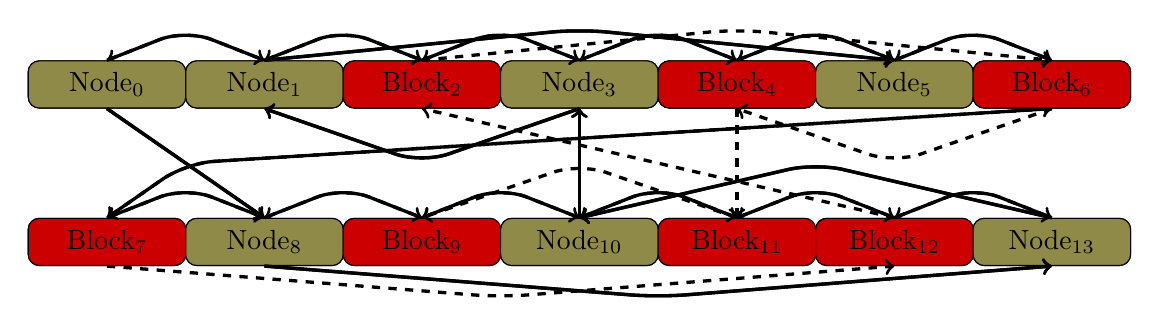
\begin{tikzpicture}[scale=1.0, rounded corners]

   \uncover<1> {
      \nodeQ (node0) at (-5.0,4) {Block$_0$};
      \nodeQ (node1) at (-3.0,4) {Block$_1$};
      \nodeQ (node2) at (-1.0,4) {Block$_2$};
      \nodeQ (node3) at (1.0,4) {Block$_3$};
      \nodeQ (node4) at (3.0,4) {Block$_4$};
      \nodeQ (node5) at (5.0,4) {Block$_5$};
      \nodeQ (node6) at (7.0,4) {Block$_6$};
      \nodeQ (node7) at (-5.0,2) {Block$_{7}$};
      \nodeQ (node8) at (-3.0,2) {Block$_{8}$};
      \nodeQ (node9) at (-1.0,2) {Block$_{9}$};
      \nodeQ (node10) at ( 1.0,2) {Block$_{10}$};
      \nodeQ (node11) at ( 3.0,2) {Block$_{11}$};
      \nodeQ (node12) at ( 5.0,2) {Block$_{12}$};
      \nodeQ (node13) at ( 7.0,2) {Block$_{13}$};

      \draw[very thick,<-, dashed, rounded corners=10pt,color=black] (node0.north) -- (-4,4.7) -- (node1.north);
      \draw[very thick,<-, dashed, rounded corners=10pt,color=black] (node1.north) -- (-2,4.7) -- (node2.north);
      \draw[very thick,<-, dashed, rounded corners=10pt,color=black] (node2.north) -- ( 0,4.7) -- (node3.north);
      \draw[very thick,<-, dashed, rounded corners=10pt,color=black] (node3.north) -- ( 2,4.7) -- (node4.north);
      \draw[very thick,<-, dashed, rounded corners=10pt,color=black] (node4.north) -- ( 4,4.7) -- (node5.north);
      \draw[very thick,<-, dashed, rounded corners=10pt,color=black] (node5.north) -- ( 6,4.7) -- (node6.north);


      \draw[very thick,<-,dashed, rounded corners=10pt,color=black] (node6.south) --  (-4,3) --  (node7.north);
      \draw[very thick,<-,dashed, rounded corners=10pt,color=black] (node7.north) --  (-4,2.7) -- (node8.north);
      \draw[very thick,<-,dashed, rounded corners=10pt,color=black] (node8.north) --  (-2,2.7) -- (node9.north);
      \draw[very thick,<-,dashed, rounded corners=10pt,color=black] (node9.north) --  ( 0,2.7) -- (node10.north);
      \draw[very thick,<-,dashed, rounded corners=10pt,color=black] (node10.north) -- ( 2,2.7) -- (node11.north);
      \draw[very thick,<-,dashed, rounded corners=10pt,color=black] (node11.north) -- ( 4,2.7) -- (node12.north);
      \draw[very thick,<-,dashed, rounded corners=10pt,color=black] (node12.north) -- ( 6,2.7) -- (node13.north);
   }

   \uncover<2-> {
      \valueQ (node0) at (-5.0,4) {Node$_0$};
      \valueQ (node1) at (-3.0,4) {Node$_1$};
      \nodeQ (node2) at (-1.0,4) {Block$_2$};
      \valueQ (node3) at (1.0,4) {Node$_3$};
      \nodeQ (node4) at (3.0,4) {Block$_4$};
      \valueQ (node5) at (5.0,4) {Node$_5$};
      \nodeQ (node6) at (7.0,4) {Block$_6$};
      \nodeQ (node7) at (-5.0,2) {Block$_{7}$};
      \valueQ (node8) at (-3.0,2) {Node$_{8}$};
      \nodeQ (node9) at (-1.0,2) {Block$_{9}$};
      \valueQ (node10) at ( 1.0,2) {Node$_{10}$};
      \nodeQ (node11) at ( 3.0,2) {Block$_{11}$};
      \nodeQ (node12) at ( 5.0,2) {Block$_{12}$};
      \valueQ (node13) at ( 7.0,2) {Node$_{13}$};
   }

   \uncover<2> {
      \draw[very thick,->,rounded corners=10pt,color=black] (node0.south) -- (node8.north);
      \draw[very thick,->,rounded corners=10pt,color=black] (node1.north) -- (1,4.7) -- (node5.north);
      \draw[very thick,->,rounded corners=10pt,color=black] (node3.south) -- (-1,3) -- (node1.south);
      \draw[very thick,->,rounded corners=10pt,color=black] (node8.south) -- (2, 1.3) -- (node13.south);
      \draw[very thick,->,rounded corners=10pt,color=black] (node10.north) -- (node3.south);
      \draw[very thick,->,rounded corners=10pt,color=black] (node13.north) -- (4,3) -- (node10.north);
   }

   \uncover<2> {
      \draw[very thick,->,dashed, rounded corners=10pt,color=black] (node2.north) -- (3,4.7) -- (node6.north);
      \draw[very thick,->,dashed, rounded corners=10pt,color=black] (node6.south) -- (5,3) -- (node4.south);
      \draw[very thick,->,dashed, rounded corners=10pt,color=black] (node4.south) -- (node11.north);
      \draw[very thick,->,dashed, rounded corners=10pt,color=black] (node11.north) -- (1,3)-- (node9.north);
      \draw[very thick,->,dashed, rounded corners=10pt,color=black] (node7.south) -- (0,1.3)-- (node12.south);
      \draw[very thick,->,dashed, rounded corners=10pt,color=black] (node12.north) -- (node2.south);
   }

   \uncover<3> {
      \draw[very thick,->,rounded corners=10pt,color=black] (node0.south) -- (node8.north);
      \draw[very thick,->,rounded corners=10pt,color=black] (node1.north) -- (1,4.7) -- (node5.north);
      \draw[very thick,->,rounded corners=10pt,color=black] (node3.south) -- (-1,3) -- (node1.south);
      \draw[very thick,->,rounded corners=10pt,color=black] (node8.south) -- (2, 1.3) -- (node13.south);
      \draw[very thick,->,rounded corners=10pt,color=black] (node10.north) -- (node3.south);
      \draw[very thick,->,rounded corners=10pt,color=black] (node13.north) -- (4,3) -- (node10.north);
   }


   \uncover<4> {
      \draw[very thick,->,rounded corners=10pt,color=black] (node0.north) -- (-4,4.7) -- (node1.north);
      \draw[very thick,->,rounded corners=10pt,color=black] (node1.north) -- (-2,4.7) -- (node2.north);
      \draw[very thick,->,rounded corners=10pt,color=black] (node2.north) -- ( 0,4.7) -- (node3.north);
      \draw[very thick,->,rounded corners=10pt,color=black] (node3.north) -- ( 2,4.7) -- (node4.north);
      \draw[very thick,->,rounded corners=10pt,color=black] (node4.north) -- ( 4,4.7) -- (node5.north);
      \draw[very thick,->,rounded corners=10pt,color=black] (node5.north) -- ( 6,4.7) -- (node6.north);
      \draw[very thick,->,rounded corners=10pt,color=black] (node6.south) --  (-4,3) --  (node7.north);
      \draw[very thick,->,rounded corners=10pt,color=black] (node7.north) --  (-4,2.7) -- (node8.north);
      \draw[very thick,->,rounded corners=10pt,color=black] (node8.north) --  (-2,2.7) -- (node9.north);
      \draw[very thick,->,rounded corners=10pt,color=black] (node9.north) --  ( 0,2.7) -- (node10.north);
      \draw[very thick,->,rounded corners=10pt,color=black] (node10.north) -- ( 2,2.7) -- (node11.north);
      \draw[very thick,->,rounded corners=10pt,color=black] (node11.north) -- ( 4,2.7) -- (node12.north);
      \draw[very thick,->,rounded corners=10pt,color=black] (node12.north) -- ( 6,2.7) -- (node13.north);
   }

\end{tikzpicture}

\end{frame}

\begin{frame}[fragile]{Alternative to pointer chasing}
Code example
\begin{itemize}
\item User provides a function to mark the \texttt{value\_type}
as {\it in use}.
\item \texttt{allocate(1)} and \texttt{deallocate(1)} calls that 
function.
\item The node type must obviously be exposed.
\end{itemize}

\begin{lstlisting}
using node_type = std::list<int>::node_type;
// Allocator configured to allocator chuncks of 256
// elements at once.
using alloc_type = node_allocator<node_type, 256>;
std::list<int, node_allocator<>> l = {1, 2, 3, 4, 5};
auto alloc = l.get_allocator();
std::copy(std::begin(alloc), std::end(alloc),
 std::ostream_iterator<node_type>(std::cout, " "))
\end{lstlisting}

\end{frame}


\subsection[Node allocation]{Node allocation}
%\begin{frame}{Illustration}{Illustration}
%
%\begin{tikzpicture}[scale=1.0, rounded corners]
%
%   \uncover<1-> {
%      \dgfile (head) at (-5,4) {Head};
%   }
%   \uncover<2-> {
%      \dgfile (node1) at (-2,4) {Node$_1$};
%      \draw[thick,->,rounded corners=10pt,color=black] (head) -- (node1);
%   }
%   \uncover<3-> {
%      \dgfile (node2) at (1,4) {Node$_2$};
%      \draw[thick,->,rounded corners=10pt,color=black] (node1) -- (node2);
%   }
%   \uncover<4-> {
%      \dgfile (node3) at (4,4) {Node$_3$};
%      \draw[thick,->,rounded corners=10pt,color=black] (node2) -- (node3);
%   }
%   \uncover<5-> {
%      \dgfile (node4) at (7,4) {Node$_4$};
%      \draw[thick,->,rounded corners=10pt,color=black] (node3) -- (node4);
%   }
%\end{tikzpicture}
%
%\end{frame}

\section[Memory Usage]{Memory Usage}

%\begin{frame}{Size reduction}{Node sizes of \texttt{std::forward\_list<int>}}
%
%\begin{enumerate}
%\item<alert@1> $N \le 256$ with $T \in [0, 256]$
%\item<alert@2> $N \le 2^{16}$ with $T \in [0, 2^{16}]$
%\item<alert@3> $N \le 2^{32}$ with $T \in [0, 2^{32}]$
%\item<alert@4> $N \le 2^{64}$ with $T \in [0, 2^{64}]$
%\end{enumerate}
%
%\begin{tikzpicture}[scale=1.0, rounded corners]
%
%   \uncover<1-> {
%      \nodeU (next) at (0.25,5) {N};
%      \valueU (value) at (0.77,5) {V};
%   }
%
%   \uncover<2-> {
%      \nodeD (next) at (0.5,4) {Next};
%      \valueD (value) at (1.6,4) {Value};
%   }
%
%   \uncover<3-> {
%      \nodeQ (next) at (1,3) {Next};
%      \valueQ (value) at (3,3) {Value};
%   }
%   \uncover<4-> {
%      \nodeO (next) at (2,2) {Next};
%      \valueO (value) at (6,2) {Value};
%   }
%\end{tikzpicture}
%
%\end{frame}

\part{How to get node allocation in the STL}

\section[Implementation]{Implementation}

\begin{frame}<beamer>{Outline}
   \tableofcontents[currentsection,currentsubsection]
\end{frame}

\subsection[Proposal]{Proposal}
\begin{frame}[fragile]{Node allocation support}

\begin{lstlisting}
template<class Alloc>
struct allocator_traits {
  // Equal to Alloc::node_allocation_only if present,
  // std::false_type otherwise. Array allocation with
  // allocate(n) is ruled out if it is std::true_type.
  using node_allocation_only = std::false_type
  // Calls a.allocate_node() if present otherwise calls
  // Alloc::allocate(1). Memory allocate with this function
  // must be deallocated with deallocate_node.
  pointer allocate_node(Alloc& a);
  // Calls a.deallocate_node(pointer) if present otherwise
  // calls Alloc::deallocate(p, 1). Can only be used with
  // memory allocated with allocate_node.
  void deallocate_node(Alloc& a, pointer p);
};
\end{lstlisting}

\end{frame}

\begin{frame}[fragile]{Node allocation implementation}

\begin{lstlisting}
pointer allocate(std::size_t /*can't handle n*/)
{
  pointer q = avail; // The next free node
  if (avail)
    avail = avail->next;

  return q;
}

void deallocate(pointer p, std::size_t /*can't handle n*/)
{
  p->next = avail;
  avail = p;
}

\end{lstlisting}

\end{frame}

\begin{frame}[fragile]{Exposing the node type}{Fancy pointers}

\begin{lstlisting}
// Cannot always hold for general A1 nd A2.
static_assert( std::is_same< std::list<T, A1>::node_type
                           , std::list<T, A2>::node_type>, "");
\end{lstlisting}

\end{frame}

\begin{frame}[fragile]{Exposing the node type}{Node type interface}

\begin{lstlisting}
template <class T, class Ptr>
struct node_type {
  using value_type = T;
  using pointer = // Usually taken from std::pointer_traits<Ptr>
  template<class U, class K>
  struct rebind { using other = node_type<U , K>; };
  // ... implementation details
\end{lstlisting}

\end{frame}

\begin{frame}[fragile]{Example}

\begin{lstlisting}
using alloc_t = rt::node_allocator<int>;
using node_type = typename std::list<int, alloc_t>::node_type;

// Buffer for 100 elements.
std::array<char, 100 * sizeof (node_type)> buffer = {{}};
alloc_t alloc(buffer);

std::list<int, alloc_t> l1(alloc);
// Inserts elements. Allocation and deallocation implemented
// with 6 lines of code.
l1 = {27, 1, 60};
...
\end{lstlisting}

\end{frame}

\subsection[Exposing the node type]{Exposing the node type}
\subsection[Node size reduction]{Node size reduction}
\subsection[Avoid pointer chasing]{Avoid pointer chasing}

\begin{frame}{Realtime node-based containers}
    \begin{columns}
        \begin{column}{0.5\textwidth}
            \texttt{std::unordered\_set}
            \begin{center}
                \includegraphics[scale=0.6]{fig/unordered_set_with_frag.pdf} \\
            \end{center}
        \end{column}

        \begin{column}{0.5\textwidth}
            \texttt{std::set}
            \begin{center}
                \includegraphics[scale=0.6]{fig/set_bench.pdf} \\
            \end{center}
        \end{column}
    \end{columns}
\end{frame}

\begin{frame}{}
    \vspace{1cm}
    \begin{center}
        {\Large \bf Thank you! Questions?} 
    \end{center}
\end{frame}

\end{document}


